\subsection{General Concepts}
\label{sec:deep_basics}

The basic building blocks of an \ac{ANN} are Artificial Neurons, which are inspired by  their biological counterparts \cite{bioneuron}.
The first artificial neuron, the perceptron, was proposed by Rosenblatt \cite{perceptron}.
The decision rule for the perceptron is described by eq. \ref{form:perceptron}.
It states that the output $\hat{y} \in \{-1, 1\}$ is defined by the sign of the dot product of a weight vector $\mathbf{w} \in \R^{n}$ with an input vector $\mathbf{x} \in \R^{n}$.
The decision boundary of this function is a linear function, which means non-linear functions like the XOR function (``exclusive or'') cannot be solved with the perceptron.

\begin{equation}
    \hat{y} = \text{sign}(\mathbf{w}^T \mathbf{x})
    \label{form:perceptron}
\end{equation}

\subsubsection{Multilayer Perceptron}

Since the perceptron is not able to solve non-linear problems. the \ac{MLP} was introduced \cite{mlp} which makes that possible.
Generally, an \ac{MLP} consists of three layer types: one input layer, one or more hidden layers, and one output layer.
The input layer is the identity function (eq. \ref{eq:identity}), which forwards the input $\textbf{x} \in \R^n$ without change to the following hidden layer.

\begin{equation}
    \text{I}(\mathbf{x}) = \mathbf{x}
    \label{eq:identity}
\end{equation}

The hidden layer, which is also called a \ac{FC} layer \cite{dl} is built out of one to $m \in \N$ perceptrons.
The output vector $\mathbf{\hat{y}} \in \R^m$ is calculated by multiplying $\mathbf{x}$ with each weight vector $\mathbf{w} \in \R^n$ and adding a constant bias vector $\mathbf{b} \in \R^m$ to the calculation \cite{dl_mit}.

\begin{equation}
    \mathbf{\hat{y}} = (\mathbf{w_1}^T\mathbf{x}, \cdots, \mathbf{w_m}^T\mathbf{x})^T + \mathbf{b}
\end{equation}

The calculation can further be simplified by using a weight matrix, which combines all weights $\mathbf{w}$ and the bias $\mathbf{b}$.
The output $\mathbf{\hat{y}}$ is then the matrix multiplication of the weight matrix $W \in \R^{(n+1) \times m}$ with the input vector $\mathbf{x}$.
The dimensionality of $\mathbf{x}$ has to be extended with a \textit{1} at the end hence results in $\mathbf{x} \in \R^{(n+1)}$ \cite{dl}.
The current output vector $\mathbf{\hat{y}}$ is just a linear transformation of the input vector $\mathbf{x}$, but biological neurons are also able to process a received signal non-linearly \cite{dl_mit}, therefore activation functions $f_{a}: \R^n \to \R^n$ are used to mimic this behavior.
Some commonly used activation functions and specifically the ones used in this thesis, are presented in section \ref{sec:activation_functions}.
Combining the activation function and the matrix multiplication results in the following formula:

\begin{equation}
    \mathbf{\hat{y}} = f_a(\mathbf{W}^T\mathbf{x})
    \label{eq:fc_weights}
\end{equation}

The last missing layer type is the output layer, which in a classification setting outputs a vector of conditional class probabilities $\mathbf{\hat{y}} \in \R^c$, where $c$ is the number of classes.
Commonly the softmax activation function is used to produce such an output \cite{softmax}.
The softmax function takes as input the output of a previous layer and outputs a vector of pseudo probabilities.
The equation \ref{eq:softmax} defines the $i$-th element of the output vector, where $C$ is the length of the input $\mathbf{x}$, which is also the number of classes to predict.

\begin{equation}
    \text{softmax}(\mathbf{x})_i = \frac{e^{x_i}}{\sum_{j=1}^Ce^{x_j}}
    \label{eq:softmax}
\end{equation}

Since the output of one layer is the input for the following layer a \ac{MLP} can be mathematically described in a chain like function structure as $f^{(O)}( f^{(h)} ( \cdots f^{(1)} (f^{(I)}(x))))$, where $f^{(I)}$ is the input layer, $f^{(O)}$ the output layer and $f^{(1)} \cdots f^{(h)}$ are the amount of $h$ hidden layers, respectively. Note that in practive several different functions can be defined as a layer.

\begin{figure}[t]
	\centering
	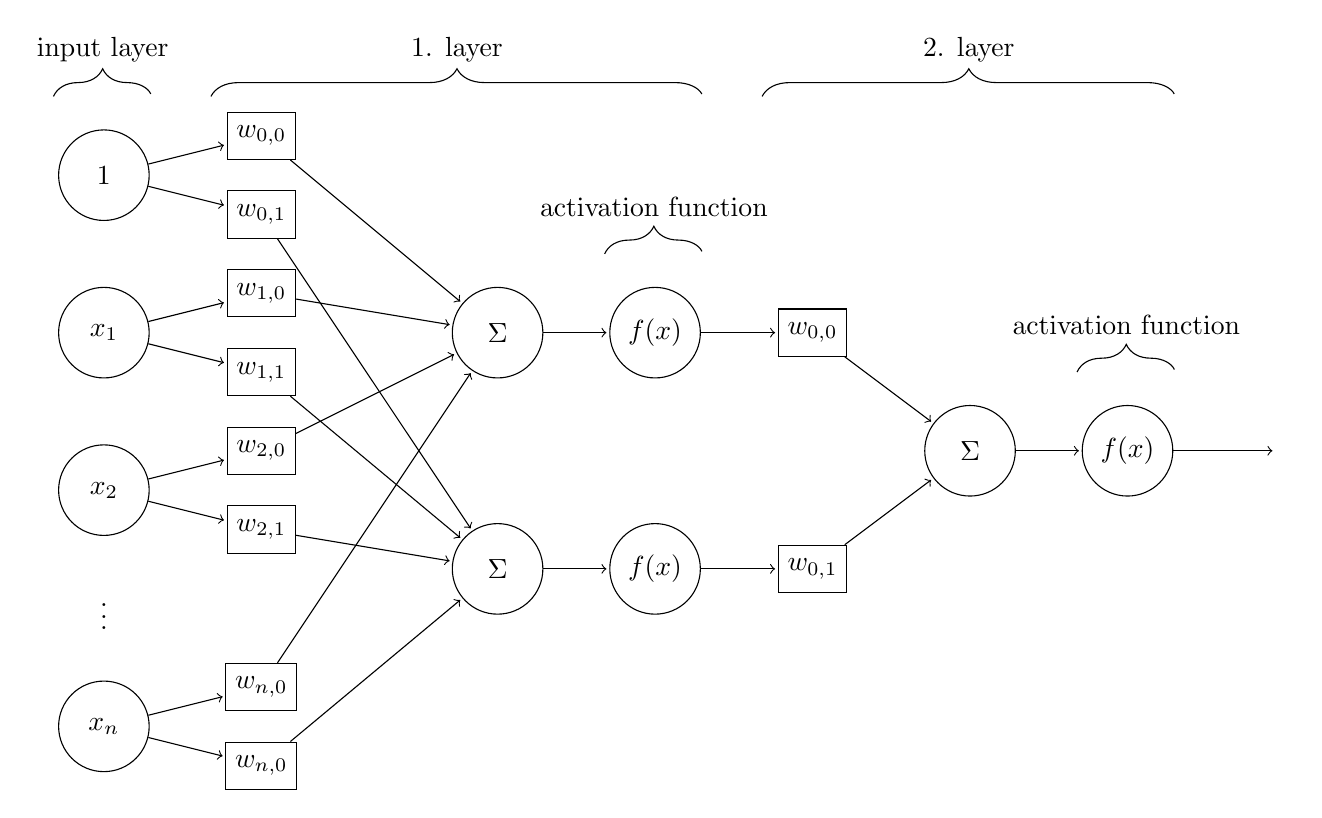
\begin{tikzpicture}[shorten >=1pt]
		\tikzstyle{unit}=[draw,shape=circle,minimum size=1.15cm]
		\tikzstyle{hidden}=[draw=none]
        \tikzstyle{weight}=[draw,shape=rectangle,minimum size=0.6cm]


        % input layer
        \node[unit](b0) at (0, 7, 0){$1$};
        \node[unit](x1) at (0, 5, 0){$x_1$};
        \node[unit](x2) at (0, 3, 0){$x_2$};
        \node at (0, 1.5){\vdots};
        \node[unit](xn) at (0, 0, 0){$x_n$};
		\draw [decorate,decoration={brace,amplitude=10pt},xshift=-4pt,yshift=0pt] (-0.5,8) -- (0.75,8) node [black,midway,yshift=+0.6cm]{input layer};

        % weight layer
        \node[weight](w00) at (2, 7.5, 0){$w_{0,0}$};
        \node[weight](w01) at (2, 6.5, 0){$w_{0,1}$};

        \node[weight](w10) at (2, 5.5, 0){$w_{1,0}$};
        \node[weight](w11) at (2, 4.5, 0){$w_{1,1}$};

        \node[weight](w20) at (2, 3.5, 0){$w_{2,0}$};
        \node[weight](w21) at (2, 2.5, 0){$w_{2,1}$};

        \node[weight](wn0) at (2, 0.5, 0){$w_{n,0}$};
        \node[weight](wn1) at (2, -0.5, 0){$w_{n,0}$};

        % sum layer
        \node[unit](sum0) at (5, 5, 0){$\Sigma$};
        \node[unit](sum1) at (5, 2, 0){$\Sigma$};

        % activation layer
        \node[unit](acti0) at (7, 5, 0){$f(x)$};
        \node[unit](acti1) at (7, 2, 0){$f(x)$};
		\draw [decorate,decoration={brace,amplitude=10pt},xshift=-4pt,yshift=0pt] (6.5,6) -- (7.75,6) node [black,midway,yshift=+0.6cm]{activation function};

		\draw [decorate,decoration={brace,amplitude=10pt},xshift=-4pt,yshift=0pt] (1.5,8) -- (7.75,8) node [black,midway,yshift=+0.6cm]{1. layer};

        % weight layer 2
        \node[weight](w200) at (9, 5, 0){$w_{0,0}$};
        \node[weight](w201) at (9, 2, 0){$w_{0,1}$};

        % sum layer 2
        \node[unit](sum2) at (11, 3.5, 0){$\Sigma$};

        % activation layer 2
        \node[unit](acti2) at (13, 3.5, 0){$f(x)$};
		\draw [decorate,decoration={brace,amplitude=10pt},xshift=-4pt,yshift=0pt] (12.5,4.5) -- (13.75,4.5) node [black,midway,yshift=+0.6cm]{activation function};


		\draw [decorate,decoration={brace,amplitude=10pt},xshift=-4pt,yshift=0pt] (8.5,8) -- (13.75,8) node [black,midway,yshift=+0.6cm]{2. layer};

        % hidden output
        \node[hidden](h0) at (15, 3.5, 0){};

        \draw[->](b0) -- (w00);
        \draw[->](b0) -- (w01);

        \draw[->](x1) -- (w10);
        \draw[->](x1) -- (w11);

        \draw[->](x2) -- (w20);
        \draw[->](x2) -- (w21);

        \draw[->](xn) -- (wn0);
        \draw[->](xn) -- (wn1);

        \draw[->](w00) -- (sum0);
        \draw[->](w10) -- (sum0);
        \draw[->](w20) -- (sum0);
        \draw[->](wn0) -- (sum0);

        \draw[->](w01) -- (sum1);
        \draw[->](w11) -- (sum1);
        \draw[->](w21) -- (sum1);
        \draw[->](wn1) -- (sum1);

        \draw[->](sum0) -- (acti0);
        \draw[->](sum1) -- (acti1);

        \draw[->](acti0) -- (w200);
        \draw[->](acti1) -- (w201);

        \draw[->](w200) -- (sum2);
        \draw[->](w201) -- (sum2);

        \draw[->](sum2) -- (acti2);
        \draw[->](acti2) -- (h0);

	\end{tikzpicture}
	\caption{Multi Layer Perceptron with two layers}
	\label{fig:mlp}
\end{figure}


\subsubsection{Learning Procedure}

In the first step, the input data is fed to the network producing an output $\mathbf{\hat{y}}$.
This step is called forward propagation and is just the above-described method of calculating the output of a layer and using it as the input for the next one.

The output $\mathbf{\hat{y}} \in \R^c$ is compared to the desired output $\mathbf{y} \in \R^c$, using a loss function $L(\mathbf{y}, \mathbf{\hat{y}}): (\R^c, \R^c) \to \R$.
The labels $\mathbf{y}$ normally are one-hot encoded, which means that a one is put at the index of the respective class and the other elements (classes) are set to zero in the label vector \cite{one_hot_enc}.

A common loss function is the \ac{MSE} \cite{yolov1}, which calculates the mean sum of the squared differences between the inputs $\mathbf{y}$ and $\mathbf{\hat{y}}$ (equation \ref{eq:mse}).

\begin{equation}
    \label{eq:mse}
    \text{MSE}(\mathbf{y}, \mathbf{\hat{y}}) = \frac{1}{C} \sum_{i=1}^{C}(y_i - \hat{y}_i)^2
\end{equation}

Another common example of a loss function would be the \ac{CE} loss (equation \ref{eq:ce}), which measures the difference between two probability distributions for a given random variable or a set of events \cite{loss_function_segmentation}.

\begin{equation}
    \label{eq:ce}
    \text{CE}(\mathbf{y}, \mathbf{\hat{y}}) = - \sum_{i=1}^C y_i \cdot log(\hat{y_i})
\end{equation}

The resulting loss value is used to calculate the gradients with respect to the weights in the last layer. Due to the above described chained function structure of an \ac{MLP} the chain rule can be used to propagate the error back through the network and calculate the gradients for all remaining layers.

After all gradients have been calculated the weights of each layer are optimized.
A simple optimizer is the stochastic gradient descent, whose update rule is defined as:

\begin{equation}
    \mathbf{W}^{(k+1)} = \mathbf{W}^{(k)} - \eta \nabla L(\mathbf{W}^{(k)})
\end{equation}

Here, $k$ denotes the current time step, $\mathbf{W}^{(k+1)}$ the updated weights, and $\mathbf{W}^{(k)}$ the current state of the weights.
The variable $\eta$ is the learning rate of the network, which scales the amount of gradient that is used to update the weights.
Typically an $0 < \eta < 1$ is chosen since big values have shown to destabilize the training process, resulting in divergence of the loss.
Further, $\nabla L(\mathbf{W}^{(k)})$ denotes here the gradients with respect to the loss function at the respective layer.

To accelerate the training the stochastic gradient descent can be extended by a momentum term \cite{sgd_momentum}.
The momentum term and the resulting update rule are defined as follows:

\begin{equation}
    \mathbf{V}^{(k)} = \mu \mathbf{V}^{(k-1)} - \eta \nabla L(\mathbf{W}^{(k)})
\end{equation}

\begin{equation}
    \mathbf{W}^{(k+1)} = \mathbf{W}^{(k)} + \mathbf{V}^{(k)}
\end{equation}

The variable $\mu$ denotes here the momentum value, which is typically set to $0.9$, $0.99$ respectively \cite{adam}.
The idea is that one can incorporate the weighted value of the previous update to accelerate in directions with persistent gradient \cite{dl}.

\subsection{Activation Functions}
\label{sec:activation_functions}

Non-linear activation functions play a crucial role in the performance of an \ac{ANN}, since this enables universal function approximation \cite{mish}.
Where universal function approximation means that any arbitrary function can be approximated.
In the perceptron the \textit{sign} function was used, but due to its non-differentiable property, it is not suited for the use in \acp{ANN}, since backpropagation requires differentiability of the activation function.
Therefore, various differentiable activation functions have been introduced.

\subsubsection{Sigmoid}

The sigmoid activation function (eq. \ref{eq:sigmoid}) is a smooth differentiable activation function, which maps its input to a $\{0, 1\}$-space.
It is commonly used in output layers since the output of the sigmoid can be interpreted as a probability.
A major drawback of the sigmoid lies in the saturating property for $\mathbf{x} \to \pm \infty$, when it's used as an activation function in trainable layers of \acp{ANN}.
Due to this the training process suffers from the so called vanishing gradient problem, where the derivative of the sigmoid tends to go towards zero and hence does not provide an update to the weights of the \ac{ANN}.

\begin{equation}
    \sigma(\mathbf{x}) = \frac{1}{1 + e^{-\mathbf{x}}}
    \label{eq:sigmoid}
\end{equation}

\subsubsection{Rectified Linear Unit (ReLU)}

The \ac{ReLU} activation function solves the gradient vanishing problem by introducing a linear term for input values $\mathbf{x} > 0$, while maintaining the non-linearity property by setting all negative input values to $0$.
The \ac{ReLU} activation function is defined as follows:

\begin{equation}
    \text{ReLU}(\mathbf{x}) =
    \begin{cases}
        \mathbf{x}, & \text{if } \mathbf{x} > 0\\
        0, & \text{else}
    \end{cases}
\end{equation}

A variation of the \ac{ReLU} activation function is the \ac{LReLU} activation function, where additionally negative values are scaled linearly.
\ac{LReLU} was introduced to tackle the dying \ac{ReLU} problem, where the network only predicts negative values and hence all gradients become zero \cite{dl}.
It is defined as follows:

\begin{equation}
    \text{LReLU}(\mathbf{x}) =
    \begin{cases}
        \mathbf{x}, & \text{if } \mathbf{x} > 0\\
        \alpha \mathbf{x}, & \text{else}
    \end{cases}
\end{equation}

\subsubsection{ReLU6}

ReLU6 is a modification of the classical \ac{ReLU}, where the output activation is limited to 6.
It is often used in resource constrained environments, especially in cases of low precision computation, since it has shown to perform robust in such cases \cite{mnetv1}.

\begin{equation}
    \text{ReLU6}(\mathbf{x}) =
    \begin{cases}
        6, & \text{if } 6 <= \mathbf{x}\\
        \mathbf{x}, & \text{if } 0 < \mathbf{x} < 6\\
        0, & \text{else}
    \end{cases}
\end{equation}

% \subsubsection{Hard Swish}

% Hard Swish \cite{mnetv3} is an approximation of the original Swish activation function, which was discovered by the researchers at Google in their extensive search for novel activation functions \cite{swish}.
% Hard Swish is calculated by multiplying the input with a piece-wise linear sigmoid approximation, the Hard Sigmoid (eq. \ref{eq:hard_sigmoid}).
% As with ReLU6, Hard Swish is used in resource constrained environments.

% \begin{equation}
%     Swish_{hard}(x) = x \sigma_{hard}(x)
% \end{equation}

% \begin{equation}
%     \sigma_{hard}(x) = \frac{ReLU6(x + 3)}{6}
%     \label{eq:hard_sigmoid}
% \end{equation}


\subsection{Convolutional Neural Networks}

While \acp{MLP} perform well on vectorial data, multidimensional data like images for example, can only be fed to a network when it was previously flattened into a vector.
One problem that arises is that when flattening for example an image of size $100 \times 100$, this would already require the input size of the network to have $10,000$ weights per neuron in the next layer.
Additionally nearby pixels in images are often highly correlated and classical unstructured \ac{ANN} fails to capture such spatial dependencies \cite{lecun_lenet}.

The proposed alternative therefor are \acfp{CNN}, which have shown to perform well over the last decade in several image related benchmarks \cite{inception} \cite{resnet} \cite{densenet}.
The classical \ac{CNN} architecture is comprised of three different layer types: convolutional layers, pooling layers and fully-connected layers.

\subsubsection{Convolutional Layer}
Convolutional layers form the major component in a \ac{CNN}.
As the name suggest the underlying mathematical foundation of those layers is the convolution operation.
The equation for a convolution in continuous space (equation \ref{eq:conv}) states that a function $f$ convolved with another function $g$, is the multiplication of those two functions, while $g$ is shifted over $f$.
The final result is then obtained by taking the integral over the whole domain \cite{dl}.

\begin{equation}
    (f * g)(x) = \int_{-\infty}^{\infty}f(\tau)g(x - \tau)d\tau
    \label{eq:conv}
\end{equation}

In deep learning the concept of convolutions is applied to an image $I \in \R^{W \times H \times C}$, where $W$ and $H$ are the width and height of the image and $C$ being the number of channels.
Further, there is a kernel $K \in \R^{k_w \times k_h \times C}$.
The image and the kernel are now convolved by moving the kernel over the image and at each position an element-wise multiplication of the overlapping area of the image and the kernel is computed.
The result is summed up and used as an output element in the convolution result.
Finally, the kernel is shifted further until the whole image has been processed.
How much pixel a kernel is shifted at a time depends on the used stride.
The higher the stride the less local information is preserved.
Typically a stride of $1$ or $2$ is used.
An example of a convolution of a $4\times4$ input with a $3\times3$ kernel and a stride of $1$ is given in figure \ref{fig:conv_example}.

\begin{figure}
\begin{center}
    \includegraphics[width=16cm]{imgs/conv/combined.png}
    \caption{Example convolution of a 4x4 input (blue) with a 3x3 kernel (dark blue) and a stride of 1, resulting in a 2x2 output (cyan) \cite{conv_arithmetic}}
    \label{fig:conv_example}
\end{center}
\end{figure}




\subsubsection{Pooling Layer}
\label{sec:max_pooling}

Pooling layers in \acp{CNN} are used to further reduce the dimensionality of the output.
During the pooling operation information across spatial locations is fused by sliding a window (typically of size $2\times2$ or $3\times3$) over the input and performing a function on the values inside the window.
In the case of max pooling the used function is the \textit{maximum} function, therefore only the maximum value inside the window is considered and used in the pooling output.
This decreases the number of parameters and hence reduces the computational cost \cite{dl}.

\subsubsection{Fully-Connected Layer}

The \ac{FC} layer as described in \ref{sec:deep_basics} is the final layer inside a \ac{CNN}.
The high-level features, which were previously build through the convolutional and max pooling layers, are flattened into a fixed size vector and passed for classification to the \ac{FC} layer.

\subsection{Batch Normalization}

A common problem while training with the \ac{ReLU} activation function is that the outputs are non-zero centered, since \ac{ReLU} is non-zero centered.
So with each layer the output distribution gets shifted from the input distribution.
This observed phenomenon is called the \textit{internal co-variate shift} and forces the network to adapt to the shifting output distribution.
The adaption produces an overhead, which is expressed in a longer training time of the network.
Therefore, Ioffe and Szegedy \cite{batchnorm} introduced \ac{BatchNorm}, a trainable layer for \acp{ANN}.
The \ac{BatchNorm} layer normalizes the feature maps along the batch axis to have zero-mean and a standard deviation of one, which not only decreases the training time, but also allows for higher learning rates and less careful initialization of the network weights.
